% 文件名:Manual.tex
% 文件描述:以 scuthesis 四川大学学位论文文档类为基础的 LaTeX 模版说明文档
% 作者:LegendaryLeo
% 修改日期:2016年6月3日
\documentclass[master,oneside,UTF8,hyperref]{../Template/scuthesis}
\usepackage{fancyvrb}
\usepackage{xcolor}
\usepackage{dirtree}
\usepackage{textcomp}
\renewcommand*{\DTstylecomment}{\color{blue}\kaishu}
\usepackage{supertabular}

\begin{document}
% 文档全局标题,用于页眉、摘要等处
\title{四川大学学位论文~\LaTeX~模版~Ver.0.10}
\ENGtitle{The SCU Dissertation \LaTeX~Ver.0.10}
% 文档封面专用标题,支持封面标题换行,使用 '\\' 命令换行
\CoverTitle{四川大学学位论文~\LaTeX~模版~Ver.0.10}

\author{Legendary L.}
\ENGauthor{Legendary L.}
\accomplishdate{\the\year~年~\the\month~月~\the\day~日}
\school{电子信息学院}
\supervisor{某某某\quad教授}
\ENGsupervisor{Prof. Anonymous}
\major{XXXX}
\ENGmajor{Something and Something}
\direction{XXXX}
\ENGdirection{XXXX}
\defensedate{XXXX~年~XX~月~XX~日}

\keywords{四川大学,论文,文档排版,\LaTeX,\CTeX}
\ENGkeywords{Sichuan University, Dissertation, Document Typesetting, \LaTeX, \CTeX}

\maketitle
\frontmatter\pagenumbering{Roman}\pagestyle{fancy}\makechaptertitlecenter
%!TEX root = ../Manual.tex
\cleardoublepage
\chapter{版权声明}
版权所有~\textcopyright~1990-\the\year~Legendary L.\footnote{Legendary Leo \url{https://github.com/cuiao}}

本文档可在~GNU~自由文档许可证(GFDL)\footnote{\url{http://www.fsf.org/licensing/licenses/fdl.html}}的第~1.3~版(或之后任意版本)或~GNU~通用公共许可证(GPL)\footnote{\url{http://www.fsf.org/licensing/licenses/gpl.html}}的第~3~版(或之后任意版本)所规定的条款下自由地复制、修改和发布。


以上所述两个许可证应该在本模版所在目录的~\verb|License/|~子目录下,文件名分别为~\verb|fdl-1.3.txt|~和~\verb|gpl-3.0.txt|。如果没有,你可以到上面提到的网址查看许可证内容。如果还不行,请写信给下面的地址以获得邮寄的许可证:
\begin{verbatim}
    The Free Software Foundation, Inc.,
    675 Mass Ave, Cambridge, MA02139, USA
\end{verbatim}

%!TEX root = ../Manual.tex
\begin{CHSabstract}
	作者本人是一名四川大学的学生,在学习科研活动中经常需要进行学术写作。在使用传统的字处理软件(如~\emph{Microsoft\textsuperscript{\textregistered} Word}~)时,由于其对数学等特殊需求的支持不够友好,因此往往会遇到各种各样的问题,无法高效地写作。作者偶然接触到了~\LaTeX~排版系统,其强大的功能、优美的数学排版和便利的自动化工具等众多优点使人印象深刻,特别适合理工科学生学习和使用。经过了解,发现国际期刊论文主要使用~\LaTeX~进行排版,且国内外许多高校均提供~\LaTeX~的学位论文模版,而我校在这方面的发展还略显不足。在这样的动机驱使下,作者在利用自己较为初级的~\LaTeX~知识,参考了北京大学~Casper Ti. Vector~同学的~\emph{pkuthss}~模版和其他相关文献的基础上,开发了~\emph{scuthesis}~这个适用于四川大学研究生使用的~\LaTeX~学位论文模版。希望此模版能够给各位同学提供一个额外的选择,模版中若有瑕疵,还请各位同学批评指正,留言、新建一个~\emph{ISSUSE}~或~\emph{FORK}~一个新分支修改。


	本文主要对~\emph{scuthesis}~文档模版的使用、功能和实现和进行了简要介绍和说明,并以自身为例进行演示。本模版在~GitHub~的链接为~\url{https://github.com/cuiao/SCU_ThesisDissertation_LaTeXTemplate}.
\end{CHSabstract}

\begin{ENGabstract}
	As a postgraduate of Sichuan University, the author of this document often needs to write academical materials in daily study and research. However, traditional word processing softwares (e.g. \emph{Microsoft\textsuperscript{\textregistered} Word} et. al.) could not provide efficient writing experience due to their lackness support for mathematics et. al. Fortunately, I accessed this \LaTeX~ system by chance and its powerful funtions, beautiful mathematic typesetting effect, the convenient automated kits et. al., which have made a great impress to me, are extremely suitable for science and engineering students. By surveying, international academic jorunals and articles mainly employing this system to typessetting. Additional, many collages and universities from both domestic and overseas are more \LaTeX-friendly by providing their offical dissertation templates in \LaTeX~ comparing with Sichuan University. Motivated by these reasons, based on my kindergarten \LaTeX~ techniques and refering to the \emph{pkuthss} and other documents, I composed this \emph{scuthesis} \LaTeX~ dissertation template for postgraduates of Sichuan University. I hope this template could provide an alternative option for your writing. If there was any flaw in this template, please leave a message to me, creat an new \emph{ISSUSE} in the repo. or \emph{FORK} a new branch to modify.


	This self-contained document is focus on a brief introduction to the using and realization of this template. The link of this template on GitHub is \url{https://github.com/cuiao/SCU_ThesisDissertation_LaTeXTemplate}.
\end{ENGabstract}

%!TEX root = ../Manual.tex
\chapter{常用缩略词表}
\emph{例:}\par
\begin{table}[ht]
	\centering
	\begin{tabular*}{\textwidth}{p{0.3\textwidth}p{0.7\textwidth}}
		TUG & \TeX~ Users Group       \\
		bib & Bibliography            \\
		bst & Bibliography Style      \\
		def & Define                  \\
		toc & Table of Contents       \\
		eps & Encapsulated PostScript \\
		cls & Class                   \\
		SCU & Sichuan University
	\end{tabular*}
\end{table}

%!TEX root = ../MainBody.tex

% 常用符号表
\chapter{常用符号表}
\begin{center}
	\begin{tabular}{p{7em}p{20em}}
		$Symbol_{1}$ & 符号$1$ \\
		$Symbol_{2}$ & 符号$2$ \\
		$Symbol_{3}$ & 符号$3$ \\
	\end{tabular}
\end{center}


\maketoc

\mainmatter\pagenumbering{arabic}\pagestyle{fancy}\makechaptertitleleft

%!TEX root = ../Manual.tex
\chapter{前言}
\label{Chap_Intro}
本文档是《四川大学学位论文~\LaTeX~模版》的说明文档。


四川大学学位论文的工作以前由~dahakawang\footnote{\url{https://github.com/dahakawang/scu_thesis_template}}~、~tan\footnote{\url{http://www.codeforge.com/article/382397}}~等人做过。本模版是在参考~Casper Ti. Vector\footnote{\url{CasperVector@gmail.com}}~~\emph{pkuthss}~模版\cite{pkuthss}的基础上完成的。


Legendary L.\footnote{Legendary Leo \url{https://github.com/cuiao}}是本文档的创建者和维护者。

\section{特点}
\label{Sect_KeyFeatures}
本模版是严格按照《四川大学硕士、博士学位论文格式》\cite{SCUDissertationFormat}中的要求编写的,有以下几个特点:
\begin{itemize}
	\item 使用简单:本模版在编写之初就考虑到~\LaTeX~初学者的情况,按照本手册的说明,不需要高深的~\LaTeX~知识便可使用本模版进行论文写作。
	\item 自动化程度高:本模版的页码、标题、题注、目录等均使用了自动化命令,一般不需要用户干预。
	\item 写作方便:本模版的主要命令在样式文件中进行了封装,并采用了多文件编译方式。方便用户的写作与修改。
\end{itemize}

\section{推荐配置}
\label{Sect_RecommandedConfiguration}
本模版的使用和正确编译依赖以下几项:
\begin{description}[style=nextline,labelindent=2em,labelwidth=!]
	\item[中文字体] 本模版需要中文字体的支持。
	\item[\TeX~发行版] 一个支持中文的~\TeX~发行版,推荐使用~\TeX~Live\footnote{\url{https://www.tug.org/texlive/}}~,本模版即是使用~\TeX~Live~构建的。
	\item[文本编辑器] 一个好用的文本编辑器有利于你的写作,推荐使用~Atom\footnote{\url{https://atom.io/}}~,必备插件为~atom-latex\footnote{\url{https://github.com/thomasjo/atom-latex}}~和~language-latex\footnote{\url{https://github.com/area/language-latex}}~。
	\item[PDF~阅读器] 一个轻量级的~PDF~阅读器有利于提升效率,推荐使用~SumatraPDF\footnote{\url{http://www.sumatrapdfreader.org/free-pdf-reader.html}}~与~atom-latex~插件联用。
\end{description}


\section{模版文件}
\label{Sect_Files}
本模版根目录\verb|./|下文件夹或文件如下:
\dirtree{%
	.1 ../.
	.2 README.md\DTcomment{自述文件}.
	.2 Template\DTcomment{模版文件夹}.
	.2 MainBody\DTcomment{论文主体文件夹}.
	.2 Manual\DTcomment{手册(本文档)文件夹}.
}
其中,\verb|Template|(模版文件夹)较为重要,一般情况下请勿修改!以下按上述文件夹分类介绍本模版中的文件。

\subsection{模版文件夹}
\label{Subsect_TemplateFolder}
\verb|Template|为本模版最重要的文件夹,用于存放本模版的样式、宏定义、资源等文件,一般情况下请勿修改!详细的文件目录如下:
\dirtree{%
	.1 Template.
	.2 scuthesis.cls\DTcomment{模版样式文件}.
	.2 scuthesis.def\DTcomment{模版宏定义文件}.
	.2 chinesebst.bst\DTcomment{中文参考文献样式文件}.
	.2 Components.
	.3 Images.
	.4 SCU{\_}TITLE.eps\DTcomment{四川大学~LOGO}.
}

\subsection{论文主体文件夹}
\label{Subsect_MainbodyFolder}
\verb|MainBody|~文件夹主要用于填写论文内容,用户可以方便地将自己的论文按照章节填写到此文件夹中。详细的文件目录如下:
\dirtree{%
	.1 MainBody.
	.2 MainBody.tex\DTcomment{主\TeX文件}.
	.2 ReferenceBase.bib\DTcomment{参考文献库文件}.
	.2 Chapters\DTcomment{章节文件夹}.
	.3 0{\_}0{\_}Abstract.tex\DTcomment{中英文摘要}.
	.3 0{\_}1{\_}Abbreviations.tex\DTcomment{缩略词表}.
	.3 0{\_}2{\_}Symbols.tex\DTcomment{符号表}.
	.3 Introduction.tex\DTcomment{引言}.
	.3 Chapter2.tex\DTcomment{第二章}.
	.3 Thanks.tex\DTcomment{致谢}.
	.3 Achievements.tex\DTcomment{科研成果}.
	.3 CopyrightAuthorization.tex\DTcomment{版权授权(请勿修改)}.
	.3 OriginalStatement.tex\DTcomment{原创声明(请勿修改)}.
}
以上文件除~\verb|CopyrightAuthorization.tex|~和~\verb|OriginalStatement.tex|~按照学校统一的内容和格式规定禁止修改外,其他均可按照用户的需要进行修改。\\
\verb|ReferenceBase.bib|~可使用~\emph{EndNote\textsuperscript{\texttrademark}}~这类文献管理工具导出。


若~\verb|Chapters|~文件夹有改动,请使用~\verb|\include{Chapters/<文件名>}|~命令在~\verb|MainBody.tex|~做相应的修改(即若在~\verb|Chapters|~中增加了文件~\verb|Chapter3.tex|~,对应在~\verb|MainBody.tex|~的命令为~\verb|%!TEX root = ../MainBody.tex

%第三章
\chapter{需求分析}
共享经济的发展如火如荼 \cite{SharingEconomy2},图书平均保有量也在稳中增长,在共享图书系统开发之前,需要具体分析用户需求,确保
符合并满足用户的需求。

\section{可行性分析}
在项目开发和需求分析之前,需要系统地分析项目开发和未来交付运行地可行性。

\begin{itemize}
	\item 市场可行性
	
	据统计分析\cite{BookMarketReport2018},2018 年中国全国图书零售市场规模维持两位数增长,2018 年
	中国图书零售市场码洋规模达894亿,同比上升 11.3\%,增速相比 2017 年有所放缓,但依然维持两位数
	增长。新书品种维持平稳,新书定价持续上升。2018 年新书平均单册码洋 41.5 元。
	
	中国图书这么庞大并且持续增长的销售规模,表明人们对于纸质书籍依然有很大的需求,而且表明
	个人手头都有一些已经购买阅读过的闲置书籍。随着纸价的上涨,图书的平均单价也在上涨,这
	也给个人获取书籍增加了不少的成本。如果能够让这些图书在消费者之间流通起来,将大大减少人们的阅读
	成本,从而使人们在相同的成本下能够阅读到更多的书籍,也提高了书籍的利用率,减少了对纸的需求,
	间接保护了生态环境。
	
	本平台将提供消费者之间图书流通的平台,让书籍在人们之间流通起来,看起来是完全可行的。

	\item 技术可行性
	
	目前,以spring开发框架进行后端开发非常流行,而且技术比较成熟,Spring 框架也使得开发 Restful
	形式的服务非常方便。Spring 还集成了 Spring JPA,Spring Security 等子模块,这大大简便了后端
	的开发。Spring 基于 POJO 的开发方式相对与企业级的 Java Bean 也非常轻量级。开发者能够快速掌握 Spring
	后端开发。笔者学习过相关技术,并且曾经使用相关技术做过一个个人博客系统。对相关技术比较了解,所以后端
	开发技术上是可行的。

	前后端分离\cite{backendDispart}的开发方式,思想也比较成熟,并且得到了广泛的应用。前后端的解耦大大加快了项目的开发效率。
	前后端可以约定交互的接口,然后同时进行开发。而且 Spring 只需要简单配置就能够开发 Restful 服务,暴露
	Restful 接口。

	Android 从最初的 Android 1.0,到当前的 Android 9.0 ,API 也非常成熟,资料文档非常齐全。Android 也有
	很多网络库和 Json 库,使得 Android 能够非常容易地访问Restful形式地服务。笔者在寒假之前就开始学习 Android 开发,
	边学习边开发,之前也尝试开发过一些 Demo,所以 Android 端技术上也是可行的。

	所以从技术地角度来讲,是完全可行的一个项目,技术非常成熟,能够迅速进行开发。
	
\end{itemize}



\section{需求概述}
主要的需求是用户的发布图书,并且浏览平台上的闲置图书,并在平台上进行个人
已发布图书基本管理,对他人图书的借阅,归还等。还包括了基础的登录注册功能。总体划分为以下几个功能
模块:

\begin{enumerate}
	\item 首页图书列表,底部包含一个导航,上面显示的是本地缓存的图书列表信息,通过上划,获取更多的图书信息。
	\item 发布图书,点击发布按钮扫描图书条形码或者手动输入图书 ISBN,最终都将图书 ISBN 作为参数,请求服务器,获取服务器返回的图书信息,
	然后用户补充图书信息,例如个人描述,出售租赁价格等,并发布图书。
	\item 最近联系人列表,显示当前用户的最近联系人列表。
	\item 我的首页,显示与我相关的信息选项,包括我的发布,我的钱包,退出登录,清除缓存等。
	\item 我的发布,显示我已经发布的图书列表。
	\item 图书详情,显示图书的详细信息,包括标题,作者,ISBN,描述,出版时间,价格等详细信息。
	\item 我的钱包,显示我的钱包余额。
	\item 注册登录,这是两个不同的界面,一个用来通过邮箱和用户名进行注册,一个用用户名或者邮箱来登录。
	\item 下订单,用户点击图书详情的购买或租赁,进行下单,并转到支付界面。
	\item 支付,用户进行支付。
\end{enumerate}

\section{用户角色}
在该系统中,用户拥有多种角色,包括用户,租书消费者,购书的消费者,书籍拥有者,交付员。当用户注册登录后,便成了该平台的用户。
当用户发布了一本图书,该用户就是一个书籍拥有者,如\cref{owner}。当该书被租出或卖出时,该用户在交付过程中可能成为交付员,如\cref{deliver},负责将图书交付给消费者。
当用户在平台上购买了某本书时该用户是购书消费者,如\cref{costumer}。当用户租了某本书时,用户是租书消费者,如\cref{costumer}。

\begin{figure}[h]
	\centering
	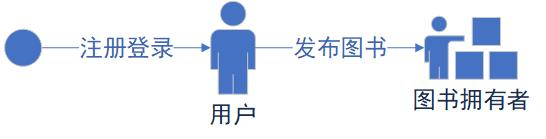
\includegraphics[scale=0.65]{Chapters/UML/owner.jpg}
	\caption{拥有者}
	\label{owner}
\end{figure}

\begin{figure}[h]
	\centering
	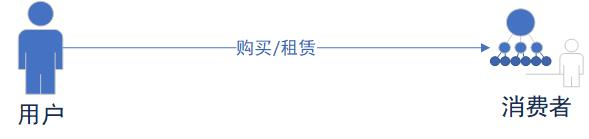
\includegraphics[scale=0.65]{Chapters/UML/costumer.jpg}
	\caption{消费者}
	\label{costumer}
\end{figure}

\begin{figure}[h]
	\centering
	
\includegraphics[scale=0.65]{Chapters/UML/deliver.jpg}
	\caption{交付员}
	\label{deliver}
\end{figure}

\section{系统业务流程}
基于 Android 的图书共享系统,需要满足用户基本的登录注册,发布图书,借阅租赁图书,沟通交流的需求。通过手机简单
的扫描图书条形码即可简单的发布图书,在手机上即可浏览图书相关信息,并且通过手机下单进行租赁,购买沟通等
功能。\cref{system_bussness_process}是完整的系统业务流程图。

\begin{enumerate}
	\item 发布图书,用户通过手机客户端扫描或手动输入图书 ISBN,获取到图书信息,进一步补充图书信息,租赁价格,出售价格,
	个人描述,点击发布。
	\item 租赁图书,用户在某本书下通过与主人沟通协商交易信息,就价格和交付方式达成一致后点击租赁,生成订单,进行支付,等待
	交付。租赁期限内,归还图书。订单完成。
	\item 购买图书,在双方协商一致后,下单,支付,交付。订单完成。
	\item 沟通交流,当用于对某本书有兴趣时,可以跟该书主人沟通交流。
\end{enumerate}

\begin{figure}[h]
	\centering
	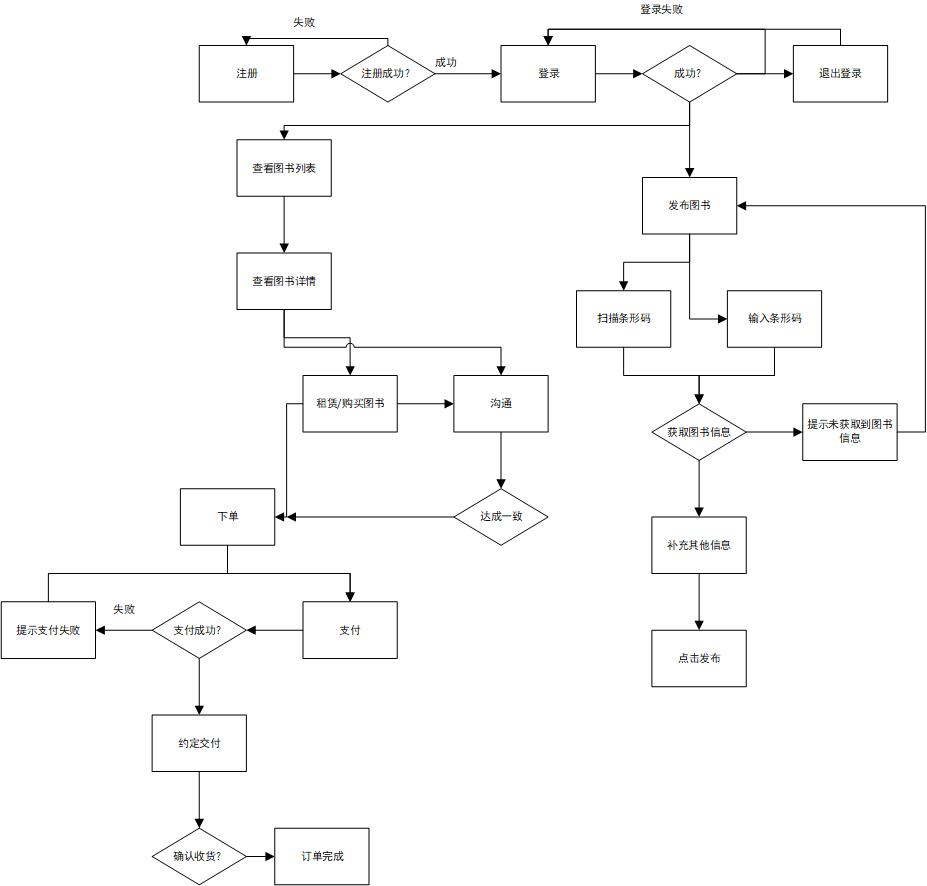
\includegraphics[scale=0.6]{Chapters/UML/system_bussness_process.jpg}
	\caption{系统业务流程图}
	\label{system_bussness_process}
\end{figure}

\section{功能需求}
\cref{function_structure}是功能结构图

\begin{figure}[h]
	\centering
	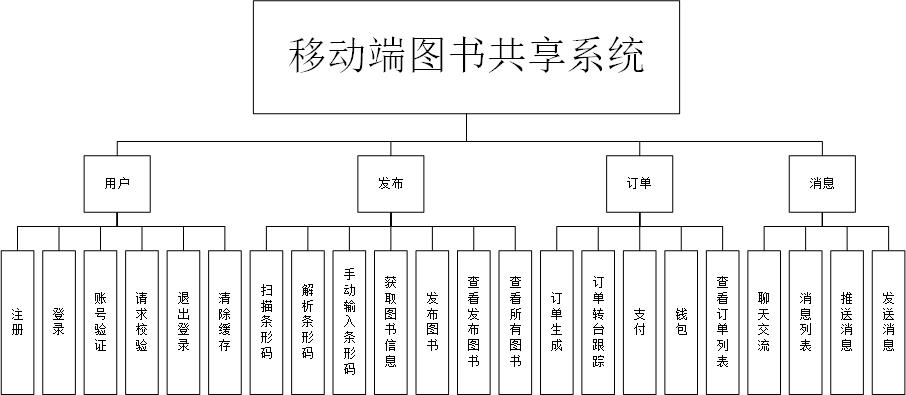
\includegraphics[scale=0.65]{Chapters/UML/function_structure.jpg}
	\caption{功能结构图}
	\label{function_structure}
\end{figure}

\begin{itemize}
	\item 注册, 客户端的用户注册。
	\item 账号验证,用户注册时验证账号是否合法。
	\item 登录,客户端用户登录。
	\item 请求校验,对用户请求的合法性进行角色权限判断。
	\item 扫描条形码,移动端调用详细扫描条形码。
	\item 解析条形码,对扫描到的条形码进行解析。
	\item 手动输入条形码,用户自行输入条形码。
	\item 获取图书信息,根据 ISBN 获取图书相关信息。
	\item 发布图书,客户端完成用户图书的发布。
	\item 订单生成,用户下单,服务器生成相应订单。
	\item 聊天交流,用户之间的沟通协商。
	\item 订单状态跟踪,对订单状态的改变。用户下订单时,订单处于未支付状态。用户支付,订单变为已支付状态。订单交付,订单变为完成状态。
	\item 支付,对订单进行支付,检查用户账户余额,并完成扣款。
	\item 钱包,对用户账户的余额进行操作,增加,扣除。
	\item 查看订单列表,获取用户完整的订单列表。
	\item 查看发布图书,获取用户的所有已发布的图书。
	\item 查看所有图书,获取所有用户发布的所有图书。
	\item 退出登录,完成用户退出操作。
	\item 清除缓存,清除客户端缓存数据。
	\item 消息列表,获取用户的聊天记录。
	\item 推送消息,用户收到来自其他人的消息时,推送消息。
	\item 发送消息,发送给其他用户消息。
\end{itemize}

\section{数据需求}

\begin{itemize}
	\item 用户账户信息,在注册和登录时,用户在客户端完成信息补充。
	\item 图书 ISBN, 通过条形码扫描解析或者用户手动输入获取 ISBN。
	\item 图书详情的 Json 数据,通过客户端获取到的 ISBN,从服务器获取 Json 数据,服务器从 books.googleapis.com 获取关于图书的 Json 数据信息。
	\item 订单数据,用户下单后,服务端应返回完整的订单信息。
	\item 订单列表,从服务器获取单个用户的所有订单信息。
	\item 聊天数据,用户登录后,从服务器获取历史信息。
	\item 钱包数据,查看用户余额。
	\item 用户图书列表,从服务器获取单个用户已发布的图书列表。
	\item 图书列表,从服务器获取所有已发布的图书列表。
\end{itemize}

\section{本章小结}
本章主要完成了共享图书的需求分析,首先对系统开发的可行性进行了分析,从经济可行性、技术可行性两个方面进行
了分析。然后对共享图书的功能需求进行了分析说明。

|~)。更多的使用方法请详见第\ref{Chap_UsingOfThisTemplate}章。

\subsection{手册文件夹}
\label{Subsect_ManualFolder}
\verb|Manual|~是本手册的文件夹,其内容与~\verb|MainBody|~较为类似,在此不做赘述。详细的文件目录如下:
\dirtree{%
	.1 Manual.
	.2 Manual.tex\DTcomment{本手册主\TeX文件}.
	.2 Manualbib.bib\DTcomment{本手册参考文献库文件}.
	.2 Manual.pdf\DTcomment{本手册}.
	.2 Chapters\DTcomment{本手册章节文件夹}.
	.3 0{\_}0{\_}Abstract.tex\DTcomment{中英文摘要}.
	.3 0{\_}1{\_}Abbreviations.tex\DTcomment{缩略词表}.
	.3 0{\_}2{\_}Symbols.tex\DTcomment{符号表}.
	.3 1{\_}Introduction.tex\DTcomment{前言(本章)}.
	.3 2{\_}Using.tex\DTcomment{模版的使用}.
	.3 3{\_}Realization.tex\DTcomment{部分功能实现}.
	.3 Thanks.tex\DTcomment{致谢}.
	.3 Achievements.tex\DTcomment{科研成果}.
	.3 CopyrightAuthorization.tex\DTcomment{版权授权(请勿修改)}.
	.3 OriginalStatement.tex\DTcomment{原创声明(请勿修改)}.
	.3 CopyrightStatement.tex\DTcomment{版权声明(请勿修改)}.
}

%!TEX root = ../Manual.tex
\chapter{模版的使用}
\label{Chap_UsingOfThisTemplate}
\section{功能}
\label{Sect_Features}
本节主要介绍本模版所依赖的类库和提供的功能/命令。
\subsection{依赖的类库}
\label{Subsect_RequiredPackages}
本模版依赖的类库/宏包(~Packages~)如\cref{table_RequiredPackages}所示:
\begin{table}[H]
	\centering
	\caption{本模版依赖的类库/宏包}
	\label{table_RequiredPackages}
	\zihao{5}
	\begin{tabular*}{\textwidth}{l@{\extracolsep{\fill}}p{0.7\textwidth}}
		\toprule
		\textbf{宏包名称} & \textbf{功能描述}     \\
		\midrule
		\verb|ctexbook|\cite{Packages_CTeX}    & \CTeX~书籍类,支持中文书籍类的~\LaTeX~框架。本模版是以此为核心构建的。\\
		\verb|ifthen|\cite{Packages_ifthen} & 提供增强型的逻辑判断功能。 \\
		\verb|graphicx|\cite{Packages_graphicx} & 提供图片插入及其增强功能,支持~pdf~、~eps~等格式。 \\
		\verb|anysize|\cite{Packages_anysize} & 支持自定义纸张大小,本模版的16开页面需此宏支持。 \\
		\verb|epstopdf|\cite{Packages_epstopdf} & 支持将~eps~转换为~pdf~,并能够跨目录访问。 \\
		\verb|hyperref|\cite{Packages_hyperref} & 支持文档导航标签及超链接功能。 \\
		\verb|cleveref|\cite{Packages_cleveref} & 支持更易使用和更灵活的交叉引用。 \\
		\verb|tocloft|\cite{Packages_tocloft} & 支持自定义目录样式。 \\
		\verb|tocbibind|\cite{Packages_tocbibind} & 支持在目录中显示参考文献、附录等项目。 \\
		\verb|caption2|\cite{Packages_caption2} & 支持自定义题注样式。 \\
		\verb|natbib|\cite{Packages_natbib} & 支持自定义参考文献编号样式,提供编号排序和分类。 \\
		\verb|enumitem|\cite{Packages_enumitem} & 支持自定义列表环境。 \\
		\verb|amsmath|\cite{Packages_amsmath} & 支持~\AmS~通用的数学表达方式。 \\
		\verb|amsfonts|\cite{Packages_amsfonts} & 支持~\AmS~通用的特殊数学字体,如~$\mathbb{C}$~、~$\mathbb{R}$~等。 \\
		\verb|amsthm|\cite{Packages_amsthm} & 支持~\AmS~通用的数学定理环境。 \\
		\verb|mathtools|\cite{Packages_mathtools} & 为~\AmS~数学表达式提供扩展,如公式的多行环境。 \\
		\verb|amssymb|\cite{Packages_amssymb} & 支持~\AmS~通用的特殊符号。 \\
		\verb|float|\cite{Packages_float} & 支持图表类浮动对象的扩展设置。 \\
		\verb|booktabs|\cite{Packages_booktabs} & 支持三线表等专业表格。 \\
		\bottomrule
	\end{tabular*}
\end{table}
\subsection{提供的选项}
\label{Subsect_ProvidedOptions}
本模版以~\verb|ctexbook|~文档类为基础,提供~\verb|<degree>|~选项用于选择学位论文类别,其余选项~\verb|<ctexbook_opt>|~均会被传递给~\verb|ctexbook|~文档类。


加载本模版定义的文档类的命令为:
\fvset{fontsize=\zihao{-5}}
\begin{Verbatim}[gobble=1,frame=single,numbers=left]
	\documentclass[<degree>,<ctexbook_opt1>,...,<ctexbook_optXX>]{../Template/scuthesis}
\end{Verbatim}
其中,~\verb|<degree>|~可用选项为~\verb|doctor|~、~\verb|master|~和~\verb|bachelor|\footnote{虽然此选项代表学士学位论文选项,但并未针对其论文格式要求作出适配。}~,分别代表博士、硕士和学士学位论文。值得注意的是,一般推荐使用~\verb|UTF-8|~编码撰写论文,因此建议设置~\verb|<ctexbook_opt1>|~为~\verb|UTF-8|~。其他有关~\verb|ctexbook|~文档类的选项请参考相关文档\cite{Packages_CTeX}。


本手册加载~\emph{scuthesis}~文档类的命令为\footnote{在需要生成阅读版论文时,即不需要在章节非奇数页时在前插入空白页是,可在~UTF8~选项前加入~oneside~选项。本手册即采用这个选项。}:

\begin{Verbatim}[gobble=1,frame=single,numbers=left]
	\documentclass[master,oneside,UTF8,hyperref]{../Template/scuthesis}
\end{Verbatim}

\subsection{提供的命令}
\label{Subsect_ProvidedCommands}
本模版提供的带参数命令如\cref{table_ProvidedCommandsWithPar}所示。这种带参数的命令一般用以下方式调用:
\fvset{fontsize=\zihao{5}}
\begin{Verbatim}[gobble=1,frame=single,numbers=left]
	\command{<parameter1>}{<parameter2>}...{<parameterXX>}
\end{Verbatim}
其中,~\verb|<parameter>|~指输入的参数,用~\verb|{ }|~包含。


\begin{center}
	\topcaption{\emph{scuthesis}~提供的带参数命令}
	\label{table_ProvidedCommandsWithPar}
	\tablefirsthead{
		\toprule
		\multicolumn{1}{l}{\textbf{命令}} & \multicolumn{1}{l}{\textbf{功能描述}}\\
		\midrule
	}
	\tablehead{
		\multicolumn{2}{l}{\emph{——~续\cref{table_ProvidedCommandsWithPar}~——}}\\
		\toprule
		\multicolumn{1}{l}{\textbf{命令}} & \multicolumn{1}{l}{\textbf{功能描述}}\\
		\midrule
	}
	\tabletail{
		\bottomrule
		\multicolumn{2}{r}{\emph{——~续表见下页~——}}\\
	}
	\tablelasttail{\bottomrule}
	\begin{supertabular*}{\textwidth}{l@{\extracolsep{\fill}}p{0.7\textwidth}}
		\verb|\title| & 设定论文中文标题\\
		\verb|\ENGtitle| & 设定论文英文标题\\
		\verb|\author| & 设定论文作者中文姓名\\
		\verb|\ENGauthor| & 设定论文作者英文姓名\\
		\verb|\accomplishdate| & 设定论文完成日期\\
		\verb|\school| & 设定所属学院\\
		\verb|\supervisor| & 设定导师中文姓名\\
		\verb|\ENGsupervisor| & 设定导师英文姓名\\
		\verb|\major| & 设定专业中文名\\
		\verb|\ENGmajor| & 设定专业英文名\\
		\verb|\direction| & 设定研究方向中文名\\
		\verb|\ENGdirection| & 设定研究方向英文名\\
		\verb|\defensedate| & 设定答辩日期\\
		\verb|\keywords| & 设定中文关键词\\
		\verb|\ENGkeywords| & 设定英文关键词\\
		\verb|\university| & 设定大学中文名称\\
		\verb|\ENGuniversity| & 设定大学英文名称\\
		\verb|\fillinblank| & 双参数命令,用于在指定字段下加特定长度的下划线。第一个参数为下划线长度,第二个参数为输出字段\\

	\end{supertabular*}
\end{center}


如需设定论文的中英文标题,则在文章正式开始前输入:
\begin{Verbatim}[gobble=1,frame=single,numbers=left]
	\title{四川大学学位论文~\LaTeX~模版 Ver. 0.1}
	\ENGtitle{The SCU Dissertation \LaTeX ~ Class Ver. 0.1}
\end{Verbatim}


如需设定论文的中英文作者姓名,则在文章正式开始前输入:
\begin{Verbatim}[gobble=1,frame=single,numbers=left]
	\author{Legendary L.}
	\ENGauthor{Legendary L.}
\end{Verbatim}


或需得到~3cm~下划线上的\fillinblank{3cm}{四川大学},需输入:
\begin{Verbatim}[gobble=1,frame=single,numbers=left]
	\fillinblank{3cm}{四川大学}
\end{Verbatim}


本模版提供的不带参数命令如\cref{table_ProvidedCommandsWithoutPar}所示:
\begin{table}[h]
	\caption{\emph{scuthesis}~提供的不带参数命令}
	\label{table_ProvidedCommandsWithoutPar}
	\begin{tabular*}{\textwidth}{l@{\extracolsep{\fill}}p{0.6\textwidth}}
		\toprule
		\textbf{命令} & \textbf{功能描述} \\
		\midrule
		\verb|\maketitle| & 根据设置字段自动生成论文封面\\
		\verb|\maketoc| & 根据章节信息自动生成目录\\
		\verb|\makechaptertitlecenter| & 使章节标题居中\\
		\verb|\makechaptertitleleft| & 使章节标题居左\\
		\verb|\autograph| & 生成如学位论文版权使用授权书样式的签名栏\\
		\bottomrule
	\end{tabular*}
\end{table}


如需生成封面,则在输入完必要信息后,使用~\verb|\maketitle|~命令生成。或若需将章节标题居左,就只需要在需要居左的章节前加~\verb|\makechaptertitleleft|,如:
\begin{Verbatim}[gobble=1,frame=single,numbers=left]
	\makechaptertitleleft	% 章节标题居左
	\chapter{绪论}		% “绪论”章节
	..............
	\chapter{问题模型的建立}	% “问题模型的建立”章节
	..............
\end{Verbatim}

\subsection{提供的环境}
\label{Subsect_ProvidedEnvironments}
本模版提供的环境如\cref{table_ProvidedEnvironments}所示。
\begin{table}[h]
	\caption{\emph{scuthesis}~提供的环境}
	\label{table_ProvidedEnvironments}
	\begin{tabular*}{\textwidth}{l@{\extracolsep{\fill}}p{0.6\textwidth}}
		\toprule
		\textbf{环境名称} & \textbf{功能描述} \\
		\midrule
		\verb|CHSabstract| & 中文摘要环境,用于填写中文摘要。\\
		\verb|ENGabstract| & 英文摘要环境,用于填写英文摘要。\\
		\verb|reference| & 参考文献环境,使自动生成的参考文献符合格式规范。\\
		\bottomrule
	\end{tabular*}
\end{table}


以上环境用以下语法在正文区使用:
\begin{Verbatim}[gobble=1,frame=single,numbers=left]
	\begin{<EnvironmentName>}
		Some text goes here...
	\end{<EnvironmentName>}
\end{Verbatim}


又比如,当需填写英文摘要时,以本手册为例:
\begin{Verbatim}[gobble=1,frame=single,numbers=left]
	\begin{ENGabstract}
		As a postgraduate of Sichuan University, the author of this
		document often needs to write academical materials in daily
		study and research. However, traditional word processing
		...........................................................
		please leave a message to me, creat an new \emph{ISSUSE} in
		the repo. or \emph{FORK} a new branch to modify.
	\end{ENGabstract}
\end{Verbatim}


\section{使用}
\label{Sect_Using}
如果您是初学者,若要正确使用本模版,需要了解一些有关~\LaTeX~的基础知识,请见\cref{Subsect_LaTeXBasics,Subsect_InsertFormula,Subsect_InsertFigureTable}。如果您能够熟练使用或对~\LaTeX~有所了解,请移步至\cref{Subsect_OtherFunctions}。
\subsection{\LaTeX~文档的基础知识}
\label{Subsect_LaTeXBasics}
一般来说,一份完整的~\LaTeX~文档可分为\emph{导言区}和\emph{正文区}两大部分,缺一不可。其中\emph{导言区}位于\emph{正文区}之前,用于加载、描述、定义或重定义文档的类型、所用到的宏包、命令、环境等。
\begin{Verbatim}[gobble=1,frame=single,numbers=left]
	% 导言区
	\documentclass[<Opt1>,<Opt2>,...,<OptN>]{<DocumentClass>}
	\usepackage[<Opt1>,<Opt2>,...,<OptN>]{<PackageName1>}
	\usepackage[<Opt1>,<Opt2>,...,<OptN>]{<PackageName2>}
	......
	% 正文区
	\begin{document}
	Your text goes here......
	\begin{<Environment1>}
		Something in <Environment1>.
	\end{<Environment1>}

	\begin{figure}[H]
		\includegraphic[scale=0.5]{<GraphicPath>}
		\caption{This is a test picture.}
		\label{fig_TestPic}
	\end{figure}
\end{document}
\end{Verbatim}


其中,导言区中的~\verb|\documentclass|~用于加载对应我文档类,要加载本模版请参见\cref{Subsect_RequiredPackages}中的描述。而~\verb|\usepackage|~用于加载特定的宏包。上文代码框中的~\verb|<Opt>|~、~\verb|<DocumentClass>|~和~\verb|<PackageName>|~分别代表\emph{选项(~Option~)}、\emph{文档类名(~Document Class Name~)}和\emph{宏包名称(~Package Name~)}。~\LaTeX~提供了很多有用的宏包,涵盖到文档排版、内容表述和文档美化等方方面面,需要的用户可以访问~\url{https://www.ctan.org/pkg}~进行浏览,或\emph{~Google LaTeX~和相应的关键字}查找。一般来说,使用默认选项对~\emph{TeX Live}~进行了安装后,会自动拥有所有的宏包。若需查看宏包的帮助文档,只需打开命令行输入~\verb|texdoc|~命令并附加所需宏包名称即可。


此外,正文区中~\verb|<Environment>|~代表文中的一个\emph{环境},使用~\verb|\begin|~和~\verb|\end|~命令包含。可以看出,整个正文区~\verb|document|~也是一个大的\emph{环境}并包括了很多子\emph{环境}。一般来说,一个~\LaTeX~文档会至少包含\emph{正文}、\emph{公式}、\emph{图}和\emph{表}等\emph{环境}。本模版除了这些基础外,还提供了如\cref{table_ProvidedEnvironments}所示的其他环境。另外,本模版集成了很多宏包,用户可以根据\cref{table_RequiredPackages}自行查阅帮助文件使用宏包提供的环境。


若想要更进一步学习~\LaTeX~的使用,推荐参考\emph{刘海洋所著《~\LaTeX~入门》}一书\cite{Book_LaTeXIntro}。

\subsection{公式}
\label{Subsect_InsertFormula}
对于理工科同学而言,~\LaTeX~的一大优势在于能够很方便地输入各种数学符号和公式。对于学位论文,一般公式按照其所在文中的位置分为\emph{行内公式}和\emph{编号公式}两种。\emph{行内公式}如~$e^{j\omega t}=\cos(\omega t)+\sin(\omega t)$~所示,位于文本行之内。而\emph{编号公式}如\cref{eqn_FourierTransform},位于文本行间或段间,且右侧有编号。
\begin{equation}
	\label{eqn_FourierTransform}
	X(j\omega)=\int_{-\infty}^{\infty}{x(t)e^{-j\omega t}}dt
\end{equation}


对于\emph{行内公式},只需在正文行中用两个~\verb|$|~将所要输入的公式内容包含即可。例如~\verb|$e^{j\omega t}=\cos(\omega t)+\sin(\omega t)$|~即为上文行内的欧拉公式。而对于\emph{编号公式},则需要在~\verb|equation|~环境中输入公式内容。\cref{eqn_FourierTransform}就是在~\verb|equation|~环境中输入的,具体内容如下所示:
\begin{Verbatim}[gobble=1,frame=single,numbers=left]
	\begin{equation}
		\label{eqn_FourierTransform}
		X(j\omega)=\int_{-\infty}^{\infty}{x(t)e^{-j\omega t}}dt
	\end{equation}
\end{Verbatim}
其中,~\verb|\begin|~和~\verb|\end|~用于界定~\verb|equation|~环境的范围,~\verb|\label|~命令用于给这个公式起一个“名字”用于交叉引用,~\verb|\omega|~为小写希腊字母~$\omega$~,~\verb|\int|~为积分号$\int$,~\verb|_{}|~和~\verb|^{}|~代表大括号中的内容分别为下标和上标,~\verb|\infty|~为符号$\infty$。


此外,对于公式的输入还有很多内容,推荐访问~\url{https://en.wikibooks.org/wiki/LaTeX/Mathematics}~以及参考\incite{Book_LaTeXIntro},获得更多信息。

\subsection{图表}
\label{Subsect_InsertFigureTable}
本模版默认加载了~\verb|graphicx|~宏包以提供在文中插入图片的功能,支持矢量(~EPS, PS, PDF~等~)和像素(~PNG, JPEG~等~)格式。使用~\verb|\includegraphics|~命令即可进行插入图片的操作。


以~\verb|..\Template\Components\Images\SCU_TITLE.eps|~为例插入图片的代码如下所示,效果如\cref{fig_SCUlogo}所示。

\fvset{fontsize=\zihao{-5}}
\begin{Verbatim}[gobble=1,frame=single,numbers=left]
	\begin{figure}[ht]
		\centering
		
\includegraphics[scale=0.3]{../Template/Components/Images/SCU_TITLE}
		\caption{“四川大学”字样(邓小平题)}
		\label{fig_SCUlogo}
	\end{figure}
\end{Verbatim}
\fvset{fontsize=\zihao{5}}

\begin{figure}[h]
	\centering
	
\includegraphics[scale=0.3]{../Template/Components/Images/SCU_TITLE}
	\caption{“四川大学”字样(邓小平题)}
	\label{fig_SCUlogo}
\end{figure}


其中,第1行~\verb|{figure}|~环境后的参数~\verb|[ht]|~用于指定这个浮动体环境的参数。表示浮动体可以出现在环境周围的文本所在处(~here~)和一页的顶部(~top~);第2行用~\verb|\centering|~表示后面的内容居中;第3行插入图片,~\verb|[scale=0.3]|~用于设置图片的尺寸;第4行使用~\verb|\caption|~给图片自动编号和设置标题;第5行的~\verb|\label|~命令给图片定义一个标签\cite{Book_LaTeXIntro},可在文中其他地方使用~\verb|\cref{}|~命令交叉引用,要引用\cref{fig_SCUlogo}只需在文中输入~\verb|\cref{fig_SCUlogo}|~即可。

\begin{table}[h]
	\centering
	\caption{傅里叶变换对}
	\label{table_FourierTransformPair}
	\begin{tabular}{ccc}
		\toprule
		\textbf{变换}    & \textbf{公式}                                                              & \textbf{备注} \\
		\midrule
		傅里叶变换    & $X(j\omega)=\int_{-\infty}^{\infty}{x(t)e^{-j\omega t}}dt$                   & 无             \\
		傅里叶反变换 & $x(t)=\frac{1}{2\pi}\int_{-\infty}^{\infty}{X(j\omega)e^{j\omega t}}d\omega$ & 无             \\
		\bottomrule
	\end{tabular}
\end{table}


\fvset{fontsize=\zihao{-6}}
\begin{Verbatim}[gobble=1,frame=single,numbers=left]
	\begin{table}[h]
		\centering
		\caption{傅里叶变换对}
		\label{table_FourierTransformPair}
		\begin{tabular}{ccc}
			\toprule
			\textbf{变换} & \textbf{公式} & \textbf{备注} \\
			\midrule
			傅里叶变换 & $X(j\omega)=\int_{-\infty}^{\infty}{x(t)e^{-j\omega t}}dt$ & 无 \\
			傅里叶反变换 & $x(t)=\frac{1}{2\pi}\int_{-\infty}^{\infty}{X(j\omega)e^{j\omega t}}d\omega$ & 无 \\
			\bottomrule
		\end{tabular}
	\end{table}
\end{Verbatim}
\fvset{fontsize=\zihao{5}}


表也是利用浮动环境~\verb|table|~插入的。~\LaTeX~可以自由绘制很多类型的表格,\cref{table_FourierTransformPair}即为常用的\emph{三线表}的一个例子,其代码如上所示。其环境参数~\verb|[h]|~与~\verb|figure|~中的定义类似。其中又嵌入了一个~\verb|tabular|~环境用于绘制表格,~\verb|tabular|~后的参数~\verb|{ccc}|~用于控制这个表格有三列且每列内容均居中。从第6行开始为表格的内容,其中~\verb|&|~用于表格列与列的分隔,~\verb|\\|~用于表格行与行之间的分隔。本模版还默认加载~\verb|booktabs|~宏包,而代码的第6、8和11行的~\verb|\toprule|~、~\verb|\midrule|~和~\verb|\bottomrule|~分别表示三线表中的顶线、中线和底线。


以上是使用本模版绘制表格的一个小例子,在实际使用中还有更多的功能和需要注意的问题,大家可参考\incite{Book_LaTeXIntro}以及对应宏包的说明文档。

\subsection{其他功能的使用}
\label{Subsect_OtherFunctions}
除了\cref{Subsect_LaTeXBasics,Subsect_InsertFormula,Subsect_InsertFigureTable}所述的基本使用方法和功能外,本模版还根据需要提供了一些经过定制后的功能,以下进行简述。
\subsubsection{交叉引用}
\label{Subsubsect_CrossRef}
一篇规范的学术文章往往会包含大量的图、表、数据或公式等资料,并且会它们层次分明地安排在文章中以便在适当的时候进行引用。因此有序、分明、自动化地组织引用这些材料一方面能够满足学术文章的写作要求,另一方面也能够给作者带来方便。本模版使用了~cleveref\cite{Packages_cleveref}~,并且针对中文的使用习惯进行了定制化。因此不仅支持自动编号待引用内容、自动识别所引内容的类型(章、节、图、表、公式等),还可以自动分类组合多个引用内容。


使用~\verb|cref|~进行交叉引用其实很简单\cite{Journal_Leo}。首先一定要确保被引用的内容被分配了一个标签(\verb|\label{<LabelName>}|,\verb|<LabelName>|为标签名,由用户自行确定),如\cref{fig_SCUlogo}代码第~5~行所示\footnote{一般使用中,在有题注~caption~时,为了避免交叉引用出现异常,需要将~label~置于~caption~之后}。

\begin{table}[ht]
	\centering
	\caption{cref~交叉引用的格式}
	\label{table_CrefFormat}
	\begin{tabular*}{\textwidth}{p{0.09\textwidth}p{0.17\textwidth}p{0.27\textwidth}p{0.47\textwidth}}
		\toprule
		\textbf{类型} & \textbf{单数格式} & \textbf{复数格式(连续)} & \textbf{复数格式(不连续)} \\
		\midrule
		章             & 第\textlangle\emph{编号}\textrangle章   & 第\textlangle\emph{编号}\textrangle~-~\textlangle\emph{编号}\textrangle章 & 第\textlangle\emph{编号}\textrangle, \textlangle\emph{编号}\textrangle~和~\textlangle\emph{编号}\textrangle章      \\
		节             & 第\textlangle\emph{编号}\textrangle节   & 第\textlangle\emph{编号}\textrangle~-~\textlangle\emph{编号}\textrangle节 & 第\textlangle\emph{编号}\textrangle, \textlangle\emph{编号}\textrangle~和~\textlangle\emph{编号}\textrangle节      \\
		小节             & 第\textlangle\emph{编号}\textrangle小节   & 第\textlangle\emph{编号}\textrangle~-~\textlangle\emph{编号}\textrangle小节 & 第\textlangle\emph{编号}\textrangle, \textlangle\emph{编号}\textrangle~和~\textlangle\emph{编号}\textrangle小节      \\
		项             & 第\textlangle\emph{编号}\textrangle项   & 第\textlangle\emph{编号}\textrangle~-~\textlangle\emph{编号}\textrangle项 & 第\textlangle\emph{编号}\textrangle, \textlangle\emph{编号}\textrangle~和~\textlangle\emph{编号}\textrangle项      \\
		页             & 第\textlangle\emph{编号}\textrangle页   & 第\textlangle\emph{编号}\textrangle~-~\textlangle\emph{编号}\textrangle页 & 第\textlangle\emph{编号}\textrangle, \textlangle\emph{编号}\textrangle~和~\textlangle\emph{编号}\textrangle页      \\
		表             & 表\textlangle\emph{编号}\textrangle   & 表\textlangle\emph{编号}\textrangle~-~\textlangle\emph{编号}\textrangle & 表\textlangle\emph{编号}\textrangle, \textlangle\emph{编号}\textrangle~和~\textlangle\emph{编号}\textrangle      \\
		图             & 图\textlangle\emph{编号}\textrangle   & 图\textlangle\emph{编号}\textrangle~-~\textlangle\emph{编号}\textrangle & 图\textlangle\emph{编号}\textrangle, \textlangle\emph{编号}\textrangle~和~\textlangle\emph{编号}\textrangle      \\
		式             & 式(\textlangle\emph{编号}\textrangle)   & 式(\textlangle\emph{编号}\textrangle)~-~(\textlangle\emph{编号}\textrangle) & 式(\textlangle\emph{编号}\textrangle),( \textlangle\emph{编号}\textrangle)~和~(\textlangle\emph{编号}\textrangle)      \\
		\bottomrule
	\end{tabular*}
\end{table}




\subsubsection{文献引用}
\label{Subsubsect_Citations}

\subsubsection{目录生成}
\label{Subsubsect_CreatTOC}

%!TEX root = ../Manual.tex
\chapter{部分功能实现}
\label{chap_Realization}


\makechaptertitlecenter
\begin{reference}
	\bibliographystyle{../Template/seuthesis}\bibliography{Manualbib}
\end{reference}

\appendix\makechaptertitleleft
%!TEX root = ../Manual.tex
\chapter{更新记录}
\label{chap_App_History}


\backmatter\makechaptertitlecenter
%!TEX root = ../MainBody.tex

% 作者在读期间科研成果简介
\chapter{作者在读期间科研成果简介}
\section*{发表论文}

\section*{承担科研项目}

%!TEX root = ../Manual.tex
\chapter{声明}
\label{Chap_OriginalStatement}
本人所呈交的学位论文是本人在导师指导下进行的研究工作及取得的研究成果。据我所知,除了本文中特别加以标注和致谢的地方外,论文中不包含其他人已经发表或撰写过的研究成果,也不包含为获得\universityname或其他教育机构的学位或证书而使用过的材料。与我一同工作的同志对本研究所做的任何贡献均已在论文中作了明确的说明并表示谢意。


本学位论文成果是本人在\universityname读书期间在导师指导下取得的,论文成果归四川大学所有,特此声明。
\vspace{4cm}
\autograph
%\begin{flushright}
%	\begin{tabular}{ll}
%		作者签字:\hspace{2cm} & 导师签字:\hspace{2cm} \\
%		日期:\hspace{2cm}       & 日期:\hspace{2cm}
%	\end{tabular}
%\end{flushright}

%!TEX root = ../Manual.tex
\chapter{学位论文版权使用授权书}
本学位论文作者完全了解\universityname有关保留、使用学位论文的规定,有权保留并向国家有关部门或机构送交论文的复印件和磁盘,允许论文被查阅和借阅。本人授权\universityname可以将学位论文的全部或部分内容编入有关数据库进行检索,可以采用影印、缩印或扫描等复制手段保持、汇编学位论文。


(保密的学位论文在解密后适用本授权书)
\vspace{4cm}
\autograph

%!TEX root = ../MainBody.tex

% 致谢
\chapter{致谢}
在做毕业设计和论文的这段时间里,非常感谢章毅老师的耐心与专业的指导。从一开始的选题,到功能的讨论,技术的选择,章毅老师给了我很多实用和专业的建议。在论文定稿前,章毅老师
还给了我很多修改意见。在章毅老师的帮助下我才完成了这份毕业设计与论文。在此,再次诚挚的感谢章毅老师对我的专业和细心指导。

\end{document}
